\subsection{\'Ordenes: Google vs PageRank vs In-Deg}
\label{subsec:exp2}
\begin{LaTeXdescription}
    \item[Objetivo] Analizar el orden obtenido respecto de otros \'ordenes
        disponibles. ¿Es igual? ¿Hay coincidencias? ¿Cu\'antas? ¿Tienen
        sentido?\\

    \item[Proposici\'on] Cualitativamente hablando, ¿c\'omo es el orden obtenido
        por PageRank? ¿Bueno? ¿Malo?. Obviamente que estas categorizaciones son
        intr\'insecas a la realidad: s\'olo nosotros podemos decir que al
        realizar una b\'usqueda web, los resultados vinieron en un orden
        correcto o deseable (es decir, lo que se buscaba en las primeras
        posiciones).  Utilizar nuestro criterio personal para hablar de la
        calidad del orden obtenido no ser\'ia muy correcto, ya que cualquier
        otra persona con criterios distintos podr\'ia disentir y ninguno de los
        criterios ser\'ia \textit{a priori} m\'as correcto que el
        otro\footnote{Se podr\'ia ver muestralmente que opina la gente de
        distintos \'ambitos, pero esto escapa al objeto de estudio de este
        trabajo.}. Pero lo que si podemos hacer es comparar el resultado
        obtenido con otros resultados disponibles, de los cuales proponemos
        In-Deg (que se basa en el grafo de conectividad) y los resultados de un
        \textit{search engine}: Google.\\

    \item[M\'etodo de Experimentaci\'on] Utilizamos la misma instancia que en el
        experimento anterior. Sobre esta instancia s\'olo nos falta calcular el
        orden In-Deg (el cual no es otra cosa que ordenar a los nodos en orden
        descendiente seg\'un su grado de entrada, es decir seg\'un la cantidad
        de ejes que los apuntan). Luego utilizamos el orden provisto por Google
        en la b\'usqueda inicial m\'as los \'ordenes obtenidos en el experimento
        previo.\\

    \item[Resultados, an\'alisis y discusi\'on]
\end{LaTeXdescription}

\begin{table}[H]
    \centering
    \caption{\'Ordenes comparativos entre los resultados de Google, PageRank e
        In-Deg}
    \label{tbl:google_pagerank_vs_indeg_siteubaar} 
    \setlength{\tabcolsep}{3pt}
    \begin{tabular}{|l|l|l|}
        \hline
        Google & PageRank & In-Deg\\
        \hline\hline
        www.derecho.uba.ar & www.agro.uba.ar & www.agro.uba.ar\\
        orga2.exp.dc.uba.ar & www.uba.ar & www.uba.ar\\
        www.agro.uba.ar & videos.agro.uba.ar & videos.agro.uba.ar\\
        www.ffyb.uba.ar & www.agro.uba.ar/cursos & www.agro.uba.ar/cursos\\
        www.uba.ar & www.agro.uba.ar/ced & www.agro.uba.ar/ced\\
        www.fvet.uba.ar & www.derecho.uba.ar & www.derecho.com.ar\\
        videos.agro.uba.ar & www.ffyb.uba.ar & www.ffyb.uba.ar\\
        iigg.sociales.uba.ar & www.fvet.uba.ar & www.fvet.uba.ar\\
        www.agro.uba.ar/cursos & orga2.exp.dc.uba.ar & orga2.exp.dc.uba.ar\\
        www.agro.uba.ar/ced & iigg.sociales.uba.ar & iigg.sociales.uba.ar\\
        \hline
    \end{tabular}
\end{table}

\par Los resultados obtenidos en \ref{tbl:google_pagerank_vs_indeg_siteubaar}
dieron resultados idénticos en cuanto a In-Deg vs PageRank, no así la búsqueda
en google, que debe utilizar otras heurísticas que no consideramos en este
trabajo. Asimismo, el orden de las búsquedas en google para un mismo término van
cambiando a lo largo del tiempo\footnote{True Story.} .\\

\par Respecto a In-Deg y PageRank, sus \'ordenes resultaron idénticos. Los
motivos por lo cual esto ocurre fueron desarrollados en el experimento anterior,
pero intuyendo que esto no tiene que ser siempre
as\'i (sino claramente PageRank no tendr\'ia sentido), realizamos un nuevo
experimento. Creamos una nueva instancia de prueba basada en los resultados de
buscar en wikipedia\cite{wikipedia} distintos t\'erminos relacionados con los
temas vistos en la materia. El grafo de conectividad resultante se puede
observar en la figura \ref{fig:wiki_graph}.

\begin{figure}[H]
    \centering
    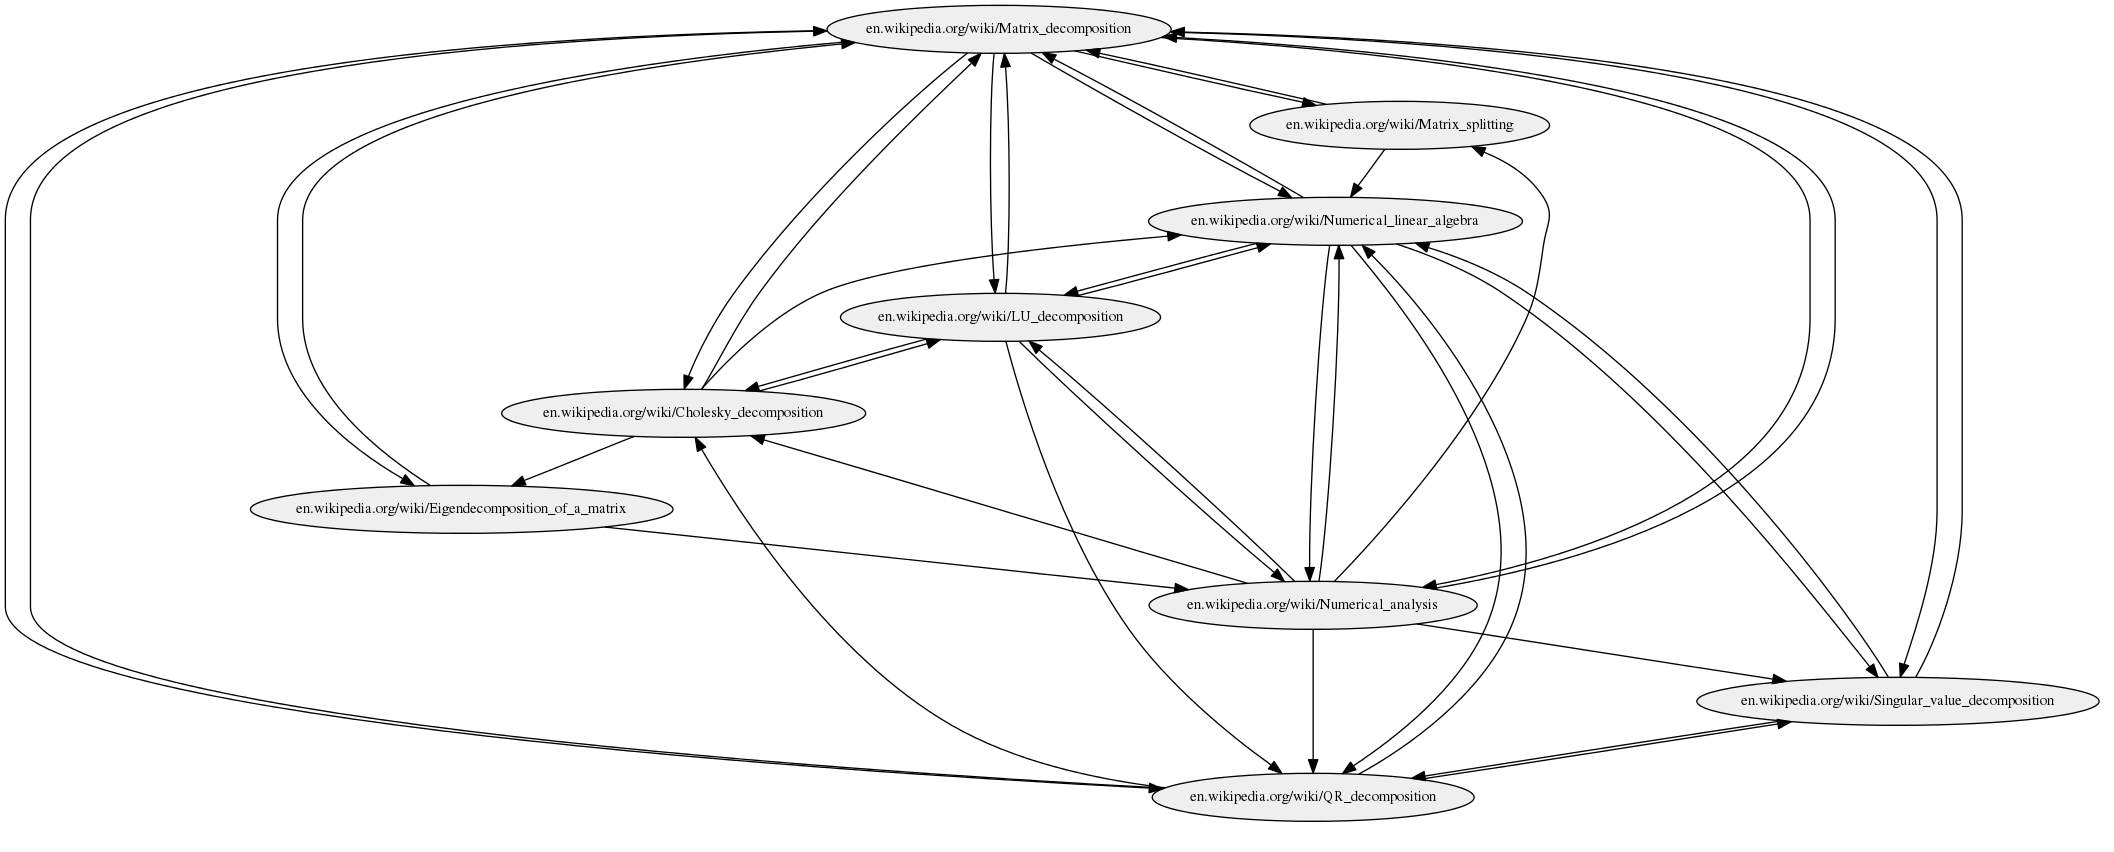
\includegraphics[width=0.75\textwidth]{exp2_conn_graph_metodos.png}
    \caption{Grafo de conectividad de p\'aginas de Wikipedia relacionadas con
        m\'etodos num\'ericos}
    \label{fig:wiki_graph}
\end{figure}

\par Sobre estas p\'aginas, calculamos los \'ordenes de PageRank e In-Deg, cuya
comparativa se encuentra detallada en el cuadro
\ref{tbl:pagerank_vs_indeg_wikipedia}. Nuevamente, In-Deg y PageRank dieron
resultados muy similares, pero no idénticos. M\'as aún, en In-Deg quedaron
varios nodos empatados, teniendo la misma cantidad de ejes entrantes. Pero esto
en PageRank no ocurri\'o, quedando definido un órden total.

\begin{table}[H]
    \centering
    \caption{\'Ordenes comparativos entre PageRank e In-Deg para Wikipedia}
    \label{tbl:pagerank_vs_indeg_wikipedia} 
    \setlength{\tabcolsep}{3pt}
    \begin{tabular}{|l|l||l|l|}
        \hline
        \multicolumn{2}{|c||}{PageRank} &\multicolumn{2}{c|}{In-Deg}\\
        \hline
        Puntaje & Nodo & Puntaje & Nodo\\
        \hline\hline
        0.196 & Matrix\_decomposition & 8 & Matrix\_decomposition\\
        0.165 & Numerical\_linear\_algebra & 7 & Numerical\_linear\_algebra\\
        0.125 & QR\_decomposition & 5 & QR\_decomposition\\
        0.106 & Numerical\_analysis & 4 & Numerical\_analysis\\
        0.105 & Singular\_value\_decomposition & 4 & LU\_decomposition\\
        0.098 & LU\_decomposition & 4 & Cholesky\_decomposition\\
        0.093 & Cholesky\_decomposition & 4 & Singular\_value\_decomposition\\
        0.057 & Eigendecomposition\_of\_a\_matrix & 2 & Eigendecomposition\_of\_a\_matrix\\
        0.050 & Matrix\_splitting & 2 & Matrix\_splitting\\
        \hline
    \end{tabular}
\end{table}

\par La diferencia entre \'ambos \'ordenes est\'a en la ubicaci\'on de
\emph{Singular value decomposition}. Mientras que en PageRank se encuentra en la
posici\'on 5, In-Deg lo lista en la 7ma ubicaci\'on. En el caso de In-Deg, la
determinaci\'on de la ubicaci\'on es determin\'istica, dependiendo del grado de
entrada del nodo que lo representa. Pero en nuestro ejemplo, vemos que existe un
empate con otros 3 nodos (como ya se ha explicado), con lo cual aqu\'i el orden
tambi\'en depende de la estabilidad y/o criterio de desempate que implemente
In-Deg. En nuestro caso, la implementaci\'on es estable, con lo cual se respeta
el orden inicial (o numeraci\'on) de los nodos. Por el otro lado, observando el
grafo podemos entender porque PageRank lo ubica en una posici\'on m\'as alta que
In-Deg: El nodo \emph{Numerical Linear Algebra}, uno de los de mayor puntaje (y
grado de entrada) tiene un link al nodo en cuesti\'on y a \emph{LU
decomposition}, pero no al resto de los valores que empatan en In-Deg. Por lo
visto en el experimento \ref{subsec:exp1}, sabemos que esto tiene un efecto de
subir el puntaje notoriamente en los nodos ''linkeados''. Luego, utilizando el
mismo razonamiento, observamos que \emph{Single value decomposition} queda por
encima de \emph{LU decomposition} por el voto/link de \emph{QR decomposition}.

\par Semánticamente, podemos observar que \textbf{en general}\footnote{\emph{QR}
queda por encima de \emph{Numerical Analysis}, creemos que esto se debe a la
morfología del grafo de referencias entre artículos en Wikipedia.} quedan
primeros en el ranking terminos mas \emph{generales} o \emph{abarcativos}; y a
medida que avanza el ranking se encuentran términos mas particulares.
Claramente, esta jerarqu\'ia de \emph{generalidad} es \'arbitraria para los
autores de este trabajo\footnote{¿Suma puntos hablar en tercera persona de
nosotros mismos? Very Scientific!}, aunque estimamos que habr\'a muy pocas
posibilidades de disenso al respecto para los temas representados por los nodos
del ejemplo.

\par Para evidenciar aún mas la diferencia entre los algoritmos de In-Deg y
PageRank decidimos alterar expl\'icitamente el grafo de conectividad de este
\'ultimo ejemplo, agregando aristas desde los 5 nodos peor puntuados hacia uno
de los últimos en el ranking In-Deg (\emph{Eigendecomposition of a matrix}).
Esto deberia aumentar drásticamente el rankeo del ultimo elemento en In-Deg ya
que aumentamos su grado de entrada en 5, pero no tanto asi en Pagerank donde la
''calidad'' de los votantes tiene una mayor injerencia. Los resultados de este
último experimento pueden verse en el cuadro
\ref{tbl:pagerank_vs_indeg_wikipedia_modificado}. 

\begin{table}[H]
    \centering
    \caption{\'Ordenes comparativos entre PageRank e In-Deg para Wikipedia con grafo alterado explícitamente}
    \label{tbl:pagerank_vs_indeg_wikipedia_modificado}
    \setlength{\tabcolsep}{3pt}
    \begin{tabular}{|l|l||l|l|}
        \hline
        \multicolumn{2}{|c||}{PageRank} &\multicolumn{2}{c|}{In-Deg}\\
        \hline
        Puntaje & Nodo & Puntaje & Nodo\\
        \hline\hline
        0.189 & Matrix\_decomposition & 8 & Matrix\_decomposition\\
        0.137 & Numerical\_linear\_algebra & 7 & Numerical\_linear\_algebra\\
        0.123 & Numerical\_analysis & 7 & Eigendecomposition\_of\_a\_matrix\\
        0.114 & Eigendecomposition\_of\_a\_matrix & 5 & QR\_decomposition\\
        0.108 & QR\_decomposition & 4 & Numerical\_analysis\\
        0.097 & Singular\_value\_decomposition & 4 & LU\_decomposition\\
        0.089 & LU\_decomposition & 4 & Cholesky\_decomposition\\
        0.087 & Cholesky\_decomposition & 4 & Singular\_value\_decomposition\\
        0.051 & Matrix\_splitting & 2 & Matrix\_splitting\\
        \hline
    \end{tabular}
\end{table}

\par Puede observarse que respecto a In-Deg el elemento con ejes entrantes
artificiales paso a ser el
tercero por su nuevo grado de entrada aumentado. En Pagerank, el elemento subió
de ranking pero quedó por debajo de Numerical\_analysis, lo cual en principio es
raro, ya que este item quedó con puntaje 4 en In-Deg. Si miramos el grafo,
veremos que, efectivamente, el hecho de que \emph{Numerical analysis} sea apuntado por
\emph{Matrix decomposition} y \emph{Numerical linear algebra}, que son los términos mas
importantes, le da mas potencia al elemento en cuestión que al elemento
\emph{Eigendecomposition of a matrix}, apuntado por los últimos 5 de la lista.

%\par Por último, vemos que en el último experimento se acentúa el orden
%\texttt{abarcativo} de los resultados respecto al dominio de los elementos.

\medskip
\par A lo largo de este experimento pudimos evidenciar las diferencias que
existen entre dos algoritmos de elaboraci\'on de rankings distintos: In-Deg y
PageRank. Esto, que no lo hab\'iamos podido exponer en el experimento previo,
nos demostr\'o el peso que PageRank le otorga a los links provenientes de
p\'aginas web con mejores puntajes, diferenciaci\'on que In-Deg no realiza.
M\'as a\'un, nos encontramos conque In-Deg parece ser tener m\'as posibilidades
de empate en su forma de ''rankear'' que PageRank, volvi\'endose dependiente del
criterio de desempate que se utilice y convirti\'endose en otra
faceta/problema a resolver, situaci\'on que puede ser despreciada en el caso de
PageRank (las probabilidades de empate ya son chicas para pocos nodos, y las
mismas son cada vez menores a mayor cantidad). Como dato de color, observamos
que los resultados devueltos por \emph{Google} son bastante distintos de los
obtenidos con PageRank, con lo cual queda claro que a pesar de haber sido este
m\'etodo un hito en la historia del motor de b\'usqueda, el mismo ya a
evolucionado much\'isimo en pocos a\~nos, lo que demuestra la importancia del
problema estudiado. 
